\documentclass[a4paper,12pt]{article}
\usepackage[utf8]{inputenc}
\usepackage[spanish]{babel}
\usepackage{color}
\usepackage{parskip}
\usepackage{graphicx}
\usepackage{multirow}
\usepackage{listings}
\usepackage{vmargin}
\usepackage{datetime}
\newdate{date}{22}{12}{2017}
\graphicspath{ {imagenes/} }
\definecolor{mygreen}{rgb}{0,0.6,0}
\definecolor{lbcolor}{rgb}{0.9,0.9,0.9}
\usepackage{epstopdf}
\usepackage{float}


\setpapersize{A4}
\setmargins{2.5cm}       % margen izquierdo
{1.5cm}                        % margen superior
{16.5cm}                      % anchura del texto
{23.42cm}                    % altura del texto
{10pt}                           % altura de los encabezados
{1cm}                           % espacio entre el texto y los encabezados
{0pt}                             % altura del pie de página
{2cm}     

\lstset{
backgroundcolor=\color{lbcolor},
    tabsize=4,    
%   rulecolor=,
    language=Java,
        basicstyle=\tiny,
        aboveskip={1.5\baselineskip},
        columns=fixed,
        showstringspaces=false,
        extendedchars=false,
        breaklines=true,
        prebreak = \raisebox{0ex}[0ex][0ex]{\ensuremath{\hookleftarrow}},
        frame=single,
        showtabs=false,
        showspaces=false,
        showstringspaces=false,
        identifierstyle=\ttfamily,
        keywordstyle=\color[rgb]{0,0,1},
        commentstyle=\color[rgb]{0.026,0.112,0.095},
        stringstyle=\color{red},
        numberstyle=\color[rgb]{0.205, 0.142, 0.73},
%        \lstdefinestyle{C++}{language=C++,style=numbers}’.
}


\begin{document}
\title{Tarea: Investigación}
\author{
Christofer Fabián Chávez Carazas \\
\small{Universidad Nacional de San Agustín de Arequipa} \\
\small{Escuela Profesional de Ciencia de la Computación} \\
\small{Computación Centrada en Redes}
}
\date{\displaydate{date}}

\maketitle

\begin{large}
 \textbf{Enunciado}
\end{large}

Realizar una investigación sobre:
\begin{itemize}
 \item API de Servlets de Java
 \item Servlets HTTP
 \item Set-Cookie
 \item Coookie
 \item Carrito de compra
\end{itemize}

\begin{enumerate}
 \item \textbf{API de Servlets de Java}
 
 Es una tecnología que nos permite crear aplicaciones web interactivas (dinámicas), es decir, le permite al usuario interactuar con la aplicación
 (hacer consultas, insertar y eliminar datos, etc).
 Un Servlet es un objeto java que pertenece a una clase que extiende de javax.servlet.http.HttpServlet.
 Son pequeños programas escritos en Java que admiten peticiones a través del protocolo HTTP. Los servlets reciben peticiones desde un navegador web,
 las procesan y devuelven una respuesta al navegador, normalmente en HTML. Para realizar estas tareas podrán utilizar las clases incluidas en el lenguaje Java.
 Estos programas son los intermediarios entre el cliente (casi siempre navegador web) y los datos (BBDD). \\
 Los servelts pueden ser incluidos en servidores que soporten la API de Servlet (ver servidores). La API no realiza suposiciones sobre el entorno que se utiliza,
 como tipo de servidor o plataforma, ni del protocolo a utilizar, aunque existe una API especial para HTTP. Los Servlets son un reemplazo efectivo para los CGI en
 los servidores que los soporten ya que proporcionan una forma de generar documentos dinámicos utilizando las ventajas de la programación en Java como conexión a
 alguna base de datos, manejo de peticiones concurrentes, programación distribuida, etc.
 Se suelen utilizar cuando:
 \begin{itemize}
  \item Las páginas web se basa en datos que proporciona el usuario. Por ejemplo, e-commerce sites.
  \item Los datos cambian frecuentemente. Por ejemplo, Webs meteorológicas.
  \item La página web utiliza información de bases de datos u otras fuentes. Por ejemplo, Aplicaciones comerciales.
 \end{itemize}
 Tienen las siguientes propiedades:
 \begin{itemize}
  \item \textbf{Manejo de Sesiones:} Se puede hacer seguimiento de usuarios a través de distintos servlets a través de la creación de sesiones.
  \item \textbf{Utilización de Cookies:} Las cookies son pequeños datos en texto plano que pueden ser guardados en el cliente. La API de servlets permite un manejo fácil y limpio de ellas.
  \item \textbf{Multi-thread:} Los servlets soportan el acceso concurrente de los clientes, aunque hay que tener especial cuidado con las variables compartidas.
  \item \textbf{Programación en Java:} Se obtienen las características de multiplataforma o acceso a APIs como JDBC, RMI, etc.
 \end{itemize}

 Los servlets utilizan clases e interfaces de dos paquetes: javax.servlet y javax.servlet.http. El paquete javax.servlet contiene clases para admitir servlets genéricos independientes
 del protocolo. Estas clases se extienden por las clases en el paquete javax.servlet.http para agregar funcionalidad específica de HTTP. El nombre del paquete de nivel
 superior es javax en lugar del familiar java, para indicar que la API del servlet es una extensión estándar.  \\
 Cada servlet debe implementar la interfaz javax.servlet.Servlet. La mayoría de los servlets se implementan extendiendo una de dos clases especiales:
 javax.servlet.GenericServlet o javax.servlet.http.HttpServlet. Un servlet independiente del protocolo es una subclase de GenericServlet, mientras que uns servlet HTTP
 es una subclase HttpServlet, que a su vez es una subclase de GenericServlet con funcionalidad adicional específica de HTTP. \\
 A diferencia de un programa Java normal, y al igual que un applet, un servlet no tiene un método \textit{main()}. En cambio, ciertos métodos de un servlet son invocados
 por el servidor en el proceso de manejo de solicitudes. Cada vez que el servidor envía una solicitud a un servlet, invoca el método \textit{service()} del servlet. \\
 Un servlet genérico debe sobre escribir su método \textit{service()} para manejar las solicitudes según corresponda para el servlet.
 
 \begin{lstlisting}
public abstract void service(ServletRequest request, ServletResponse response)
         throws ServletException, java.io.IOException
 \end{lstlisting}

 
 El método \textit{service()} acepta dos parámetros: un objeto de solicitud y un objeto de respuesta. 
 El objeto de solicitud le dice al servlet acerca de la solicitud, mientras que el objeto de respuesta se usa para devolver una respuesta.
 En la siguiente figura se muestra a una servlet genérico manejando una petición.
 
 \begin{figure}[H]
  \centering
  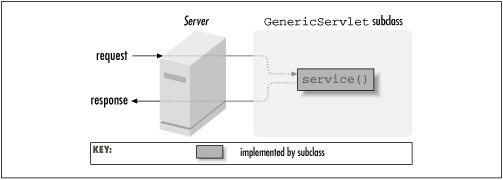
\includegraphics[scale = 0.7]{1.png}
  \caption{Un servlet genérico manejando una petición}
 \end{figure}

 \item \textbf{Servlets HTTP}
 
 Se se quiere crear un Servlet HTTP se debe extender la clase javax.servlet.http.HttpServlet. A diferencia del servlet genérico, el servlet HTTP no sobre escribe
 el método \textit{service()} En cambio debe sobre escribir al menos uno de los siguientes métodos:
 
 \begin{itemize}
  \item \textbf{doGet():} El método service del servlet llama a este método para gestionar la solicitud HTTP GET del cliente. El método Get se utiliza para obtener
  información del servidor.
  \item \textbf{doPost():} Se utiliza para enviar información al servidor.
  \item \textbf{doPut():} Este método es similar al \textit{doPost} pero con la diferencia de que se envía archivos al servidor en vez de información.
  \item \textbf{doDelete():} Permite que un cliente elimine un documento, página web o información del servidor.
  \item \textbf{init() y destroy():} Se utilizan para administrar recursos que se mantienen durante la vida del servlet.
  \item \textbf{getServletInfo():} Devuelve información sobre el servlet como el autor, la versión y derechos de autor.
 \end{itemize}

 En la siguiente figura se muestra un servlet HTTP manejando peticiones GET y POST:
 
 \begin{figure}[H]
  \centering
  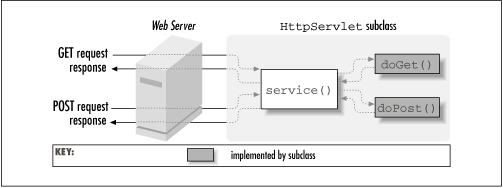
\includegraphics[scale = 0.7]{2.png}
  \caption{Servlet Http manejando peticiones GET y POST}
 \end{figure}
 
 Un pequeño servlet de ejemplo es el siguiente:
 
 \begin{lstlisting}
public class SimpleServlet extends HttpServlet {

    // Maneja el método GET de HTPP para 
    // construir una sencilla pagina Web.

    public void doGet (HttpServletRequest request, HttpServletResponse response)
              throws ServletException, IOException {
    PrintWriter out;
    String title = "Simple Servlet Output";

    // primero selecciona el tipo de contenidos y otros campos de cabecera de la respuesta
    response.setContentType("text/html");
    // Luego escribe los datos de la respuesta
    out = response.getWriter();
    out.println("<HTML><HEAD><TITLE>");
    out.println(title);
    out.println("</TITLE></HEAD><BODY>");
    out.println("<H1>" + title + "</H1>");
    out.println("<P>This is output from SimpleServlet.");
    out.println("</BODY></HTML>");
    out.close();
    }
}
 \end{lstlisting}

 Este método recibe los parámetros dados por el cliente a través de la clase \textit{HttpServletRequest} y encapsula la respuesta que se le dará al cliente a 
 través de la clase \textit{HttpServletResponse}. El servlet puede retornar al cliente cualquier tipo de información, desde texto plano hasta un ejecutable, por lo que
 es necesario señalar inicialmente qué tipo de respuesta se dará a través del método \textit{setContentType}. Luego se obtiene el objeto para poder escribir texto
 al cliente a través del método \textit{getWriter} con el cual se puede retornar una página web llamado sucesivamente el método \textit{println} hasta
 terminar con \textit{close}.

 \item \textbf{Set-Cookie}
 
 La cabecera de respuesta HTTP Set-Cookie se usa para enviar cookies desde el servidor al agente de usuario. Tiene las siguiente sintaxis:
 $$Set-Cookie:\:<cookie-name>=<cookie-value>;\:<directives> $$
 
 Las directivas disponibles son las siguientes:
 
 \begin{itemize}
  \item $<$cookie-name$>$=$<$cookie-value$>$
  
  Una cookie comienza con un par nombre-valor:
  \begin{itemize}
   \item Un $<$cookie-name$>$ puede ser cualquier cosa excepto caracteres de control (CTLs) o espacios y tabulaciones. Tampoco debe contener caracteres de separación.
   \item Para un $<$cookie-value$>$ Se permite usar cualquier caracter US-ASCII excluyendo CTLs, espacios en blanco, comillas dobles, comas, punto y coma y la barra invertida.
   \item \textbf{Prefijo \_\_Secure-:} Para cookies provenientes de páginas HTTPS.
   \item \textbf{Prefijo \_\_Host-:} Para cookies provenientes de páginas HTTPS y no son enviadas a subdominios.
  \end{itemize}
  \item Expires=$<$date$>$
  
  El tiempo de vida útil máxima de la cookie. Si no se especifica, la cookie tendrá la vida útil de una cookie de sesión, es decir, la cookie se eliminará cuando se cierra
  la sesión.
  
  \item Max-Age=$<$non-zero-digit$>$
  
  Número segundos hasta que la cookie expira.
  
  \item Domain=$<$domain-value$>$
  
  Se especifica los hosts a los que se envía la cookie. Si no se especifica, se establece de manera predeterminada en la parte del host de la ubicación del documento actual.
  
  \item Path=$<$path-value$>$
  
  Indica una ruta de URL que debe existir en el recurso solicitado antes de enviar el encabezado de Cookie.
  
  \item HttpOnly
  
  Las cookies HTTP-only no son accesibles a través de JavaScript a través de la propiedad Document.cookie, las API XMLHttpRequest y Request para mitigar ataques contra scripts de sitios cruzados (XSS).
 \end{itemize}

 \item \textbf{Cookie}
 
 Una cookie es un fichero que se descarga en un ordenador al acceder a determinadas páginas web. Las cookies permiten a una página web, entre otras cosas,
 almacenar y recuperar información sobre los hábitos de navegación de un usuario o de su equipo y, dependiendo de la información que contengan y de la forma en que
 utilice el equipo, pueden utilizarse para reconocer la sesión del usuario. En general pueden hacer lo siguiente:
 
 \begin{itemize}
  \item Recordar el usuario y contraseña en una página web.
  \item Mostrar publicidad online en función de tus intereses.
  \item Obtener estadísticas para un webmaster.
  \item Recordar preferencias en una web.
  \item Compartir en redes sociales.
  \item Llenar un carrito de compra en una tienda online.
 \end{itemize}

 En la siguiente imagen se muestra un ejemplo de lo que ocurre cuando se crean cookies en el cliente y el servidor.
 
 \begin{figure}[H]
  \centering
  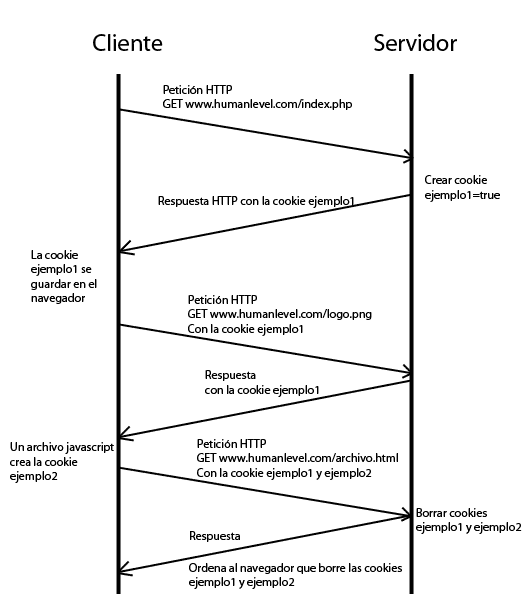
\includegraphics[scale = 0.5]{3.png}
 \end{figure}

 Las cookies se pueden dividir en diferentes tipos:
 
 \begin{itemize}
  \item \textbf{Según quien las gestione:}
  \begin{itemize}
   \item \textbf{Cookies Propias:} Son aquellas que se envían al equipo terminal del usuario desde un equipo o dominio gestionado por el propio editor y
   desde que se presta el servicio solicitado por el usuario.
   \item \textbf{Cookies de Terceros:}  Son aquellas que se envían al equipo terminal del usuario desde un equipo o dominio que no es gestionado por el editor,
   sino por otra entidad que trata los datos obtenidos a través de las cookies.
  \end{itemize}
  \item \textbf{Según su finalidad:}
  \begin{itemize}
   \item \textbf{Cookies Técnicas:}  Son aquellas que permiten al usuario la navegación a través de la página web, plataforma o aplicación y la utilización de
   las diferentes opciones o servicios que en ella existen.
   \item \textbf{Cookies de Análisis:} Son aquellas que permiten al responsable de las mismas, el seguimiento y análisis del comportamiento de los usuarios de los
   sitios web a los que están vinculadas.
  \end{itemize}
  \item \textbf{Según su tiempo de vida:}
  \begin{itemize}
   \item \textbf{Cookies de Sesión:}  Son las diseñadas para recabar y almacenar datos mientras el usuario accede a una página web. Se suelen emplear para la prestación
   del servicio solicitado por el usuario en una sola ocasión y se elimina cuando el usuario cierra la sesión.
   \item \textbf{Cookies Persistentes:} Son las diseñadas para que los datos sigan almacenados en el terminal y pueden ser accedidos y tratados durante un periodo
   definido por el responsable de la cookie, y que puede ir de unos minutos a varios años
  \end{itemize}
 \end{itemize}

 \item \textbf{Carrito de compra}
 
 Desde que Internet se convirtió en un escenario vital para las ventas y el marketing, la tecnología web se ha orientado en los últimos tiempos a potenciar
 y adecuar sus herramientas para hacer de los negocios online una alternativa fiable y productiva. En ese sentido, ningún recurso tan efectivo como el carrito de compras
 para viabilizar el comercio virtual y poner a empresas y clientes en un nuevo nivel de acercamiento. 
 
 Las 4 fortalezas o características principales de la mercadotecnia en Internet:
 
 \begin{itemize}
  \item \textbf{Flujo:} Denominado así porque genera una relación constante entre ambas partes. Según Fleming, flujo es “el estado mental en que entra un usuario de Internet
  al sumergirse en una web que le ofrece una experiencia llena de interactividad y valor añadido”. Tal suma de sensaciones propicia una mayor facilidad de acercamiento 
  entre las partes, potenciando las oportunidades de alcance de contenidos y ofrecer productos. Todo entra por la vista.
  \item \textbf{Funcionalidad:} Porque la oportunidad de acercarse hace posible un futuro proceso de venta. Si el cliente ha entrado en estado de flujo, quiere decir
  que está en camino de ser captado, pero para que el flujo de la relación no se rompa, queda dotar a la presencia on-line de funcionalidad, es decir, construir
  páginas atractivas, con navegación clara y útiles para el usuario. En posteos anteriores, hemos hablado de aquello, es decir, de la necesidad de construir websites
  visibles al usuario maximizando su experiencia de usuario para fidelizarlo. Para una tienda online resulta imprescindible este atributo.
  \item \textbf{Feedback:} Porque permite el interés e intercambio de información. El usuario está en estado de flujo y no se exaspera en su navegación, por lo que 
  las opciones de elegir el carrito de compras crecen. El website da entonces la oportunidad de preguntar al cliente qué le gusta y qué le gustaría mejorar, y 
  nutrirse de esa información para mejorar. Dialogar con el cliente para conocerlo mejor y construir una relación basada en sus necesidades refuerza el feedback, 
  probablemente, una de las mayores fortalezas de este negocio.
  \item \textbf{Fidelización:} Porque permite un vínculo duradero y especial. Internet y sus recursos de comercio virtual ofrecen la creación de comunidades de usuarios
  que aporten contenidos de manera que se establezca un diálogo personalizado con los clientes, quienes podrán ser así más fieles. Eso es lo que a la larga, buscan
  todas las tiendas virtuales. Conseguir clientes fieles y dispuestos a comprar.
 \end{itemize}

 
\end{enumerate}

\begin{thebibliography}{1}
 \bibitem{1}
 Los Teatinos, ``¿Qué es un Servlet?'', http://losteatinos.com/servlets/servlet.html
 \bibitem{2}
 Mperez, ``Java: Servlets'', Diseño de aplicaciones web.
 \bibitem{3}
 Juan Manuel Barrios, ``Java Servlets'', (2001).
 \bibitem{4}
 O'Reilly \& Associates, ``Java Servlet Programming'', (2001)
 \bibitem{5}
 CHAITANYA SINGH, ``Servlet API''
 \bibitem{6}
 ``Set-Cookie'', MDN web docs, https://developer.mozilla.org/es/docs/Web/HTTP/Headers/Set-Cookie
 \bibitem{7}
 Ramón Saquete, ``¿Qué son y cómo funcionan las cookies?'', HumanLevel (2013)
\end{thebibliography}
 

 
\end{document}

